\section{Introduction}
\subsection{Starting position}
The company PlanFabrik GmbH creates floor plans for house technology. In a first
step, the plans are analysed and enhanced through an employee. He adds more
information to the plan, like room polygons or he marks areas, where house technology
can be installed and where not. Those areas are defined by different features. For example, usually the area close to windows has a higher density of pipes, emitting heat to the room. This is to compensate the heat loss that usually occurs on windows.
\\
The process of drawing those areas is currently tool supported, but still takes a lot of time, equal to the rising amount of rooms the employee has to analyze. The idea is to create a more automated system, which does require only a small amount of user input.

\subsection{Problem description}
\label{sub:ProblemDescription}
It takes the user a lot of time to manually create all the room-areas. This is due to the fact that he has to click every corner of each room to create a room-enclosing polygon. The fact that the current tool is not very precise, which means that errors in selecting the exact corner occur regularly. The user then has to rearrange the created corner, to fit the exact corner in the image. This process of selecting all the corners by hand is highly inefficient, especially for floor plans that have several hundred or even thousands of corners in it.
\\
An automated solution would provide a faster and more comfortable solution for the client. Additionally, the software may provide additional information that is needed. It can calculate the size of each room directly, which would otherwise have to be calculated by hand.

\subsection{Goals}
The idea of theory of this bachelor thesis is to compare different algorithms, which can automatically analyse floor plans and draw the polygons for the rooms. The goal in the end is to show and explain a way to solve the problem and decide which algorithms are used best. All of this will help us create a software that can do the automated analysis for basic floor plans. More complicated floor plans may hold problems that our algorithms can not find, those are supposed to be solved manually within an editor.
\\
In the end, the program is supposed to create an output-file with the information of the areas found, which is exportable to the existing software that currently handles the following processes.

\subsection{State of the art}
This section will explain how the current process for room recognition work at the Planfabrik GmbH. It will show the actual process that is to be replaced by the software described in this work. In an additional section, there will be a description of papers similar to this one. The idea is to show what solutions are already implemented which solve the problem. It also describes the work that was the foundation for our work.

\subsubsection{Manual process}
 The process for room and zone detection is done by hand. To start, they have an unprocessed architectural floor plan in a DWG or DXF format. It is processed by the \gls{gloss:CAD}. When defining the room size, the person processing the plan has to select the edge selection tool to create the room polygon. As a room has at least three corners, this process will take at least three mouse clicks for every room. This selection tool has its difficulties, as the person operating might not select the exact corner or miss-click, which leads to the loss of the whole selected polygon. From what we have experienced, every 8-16 corners there is going to be such an inaccuracy.
 
 To define the zones for different density of heating pipes, the same process of selecting a polygon is done. Depending on the elements of the plan, this can double the amount of user interactions. Some rooms might not contain those zones but others might have several.
 
 As a result the \gls{gloss:CAD} can calculate all the different sizes of the rooms.
 
\subsubsection{Similar works}
This section introduces two papers \textit{A System to Detect Rooms in Architectural Floor Plan Images} \citep{mace_valveny_loctea_tabbone_2010} and \textit{Automatic Room Detection and Room Labeling from Architectural Floor Plans} \citep{ahmed_liwicki_weber_dengel_2012} which are two very recent paper on the exact problem of room segmentation. 

The second paper, written by Ahmed, Liwicki,Weber and Dengel, proposes a general structure for detecting floor plans. This structure will help us separate and compare the steps of the algorithms proposed in both of the discussed papers. It will also be used for the further structure of this document. They propose to separate the algorithm in three parts: \textit{Information segmentation}, \textit{Structural analysis} and \textit{Semantic analysis}. The information segmentation part contains all algorithms separating information (text, line thickness, symbols, etc.). The structural analysis contains algorithms that combine the important information from previous algorithms and and create a basic wall image. Finally the semantic analysis finds symbols and rooms based on information from the structural analysis.

The paper written by Mace, Valveny, Loctea and Tabbone uses several algorithms for information segmentation. They do a graphic/text separation because not all floor plan contain text. Therefore text like room names can not be used and have to be removed. Additionally they use a thick/thin line separation algorithm to separate the walls from the other lines of the floor plan. The walls are expected to be the thickest lines on the plan.

For structural analysis they use the hough transformation, which is described in Section \ref{subsubsec:Hough transformation}, in combination with image vectorization. This is used for a simple wall detection algorithm. The wall detection works on an image of the contour of the walls. They take two lines that are close together and have the same orientation and check if the pixels in between those lines are black. If so this is an actual wall due to the fact that before taking the contour of the walls they were connected. 

The room detection in the semantic analysis is done with a polygon partitioning technique, that uses the wall as a convex hull and tries to split it up in smaller polygons (rooms), that all have to be convex. This, in combination with the fact that rooms are mostly rectangular shape, which is adjusted during post-processing, will detect the rooms.

\begin{figure}[H]
	\centering
	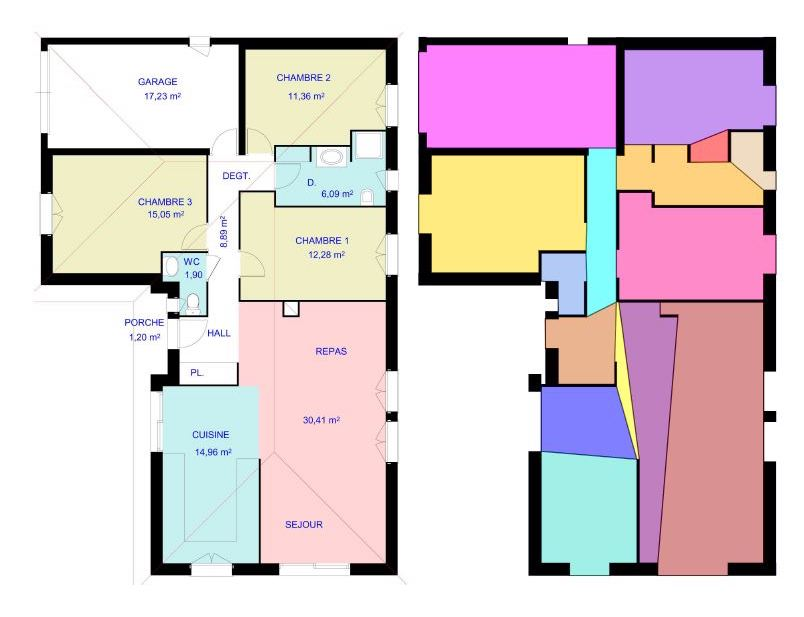
\includegraphics[width=1.0\textwidth]{paper1_floorplan}
	\caption{Room segmentation with the algorithm used in \textit{A System to Detect Rooms in Architectural Floor Plan Images} by Mace, Valveny, Loctea and Tabbone. }
	\label{fig:paper1_floorplan}
\end{figure}

The second paper mentioned above by Ahmed, Liwicki, Weber and Dengel, takes a similar approach. For information segmentation they also separate text/lines as well as separate thick/thin lines. The difference is that they use the text to name the rooms. Additionally they separate the image in thick, medium and thin lines instead of just thick and thin. Thick lines represent external, medium internal walls and thin lines represent symbols.

For structural analysis they also use a similar approach for wall detection but additionally close additional gaps with a convex/concave hypothesis, further described in the paper. Those algorithms lead to a very refined image of the walls, with better results than proposed in the previous paper.

For the semantic analysis they use \gls{gloss:SURF} as a algorithm to detect doors. This helps separating rooms, because the the definition of separation is, that there has to be a door connecting them. To find the rooms, a connected component analysis is used on the wall image. Gaps where a doors should exist, are closed with \gls{gloss:SURF} and therefore rooms are defined by a connected component. Each of these rooms will then be labeled with a name from the text layer, that overlap into the area of the detected room.

\begin{figure}[H]
	\centering
	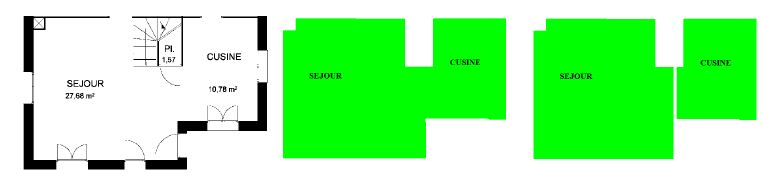
\includegraphics[width=1.0\textwidth]{paper2_floorplan}
	\caption{Room segmentation with the algorithm used in \textit{Automatic Room Detection and Room Labeling from Architectural Floor Plans} by Ahmed, Liwicki, Weber and Dengel. }
	\label{fig:paper2_floorplan}
\end{figure}

Both of those papers have a room detection rate between 80-90\%. The important part though is the room recognition rate which is only around 50\% for the work by Mace, Valveny, Loctea and Tabbone. This is really low for a real world use-case. The work by Ahmed, Liwicki, Weber and Dengel improves this rate up to about 80\%, which is a big improvement. This is most likely due to the fact that they use \gls{gloss:SURF} as a door recognition algorithm, which helps separating the rooms more accurately. Both works struggle with the difference, in how symbols and walls are depicted in architectural floor plans. They can only detect those rooms, if the walls are the thickest lines on a plan and there is no interference from symbols.
 

\subsection{Metrics}
To have a measurement, to compare our product to what is already in place at the Planfabrik GmbH, we went there and collected two values. Those values are the time which is needed to do the room segmentation and how many mouse-clicks it would take. We did that on five different floor plans, that were preselected by us. They were selected after the difficulty to analyse, rated by ourself, as well as their difference in the number of rooms.

The plans chosen are the following:

AN\_1
50er
A1\_OG



The time was taken with a countdown clock on an iPhone and was stopped manually by hand. This led to a time deviation of usually 1-2 seconds longer than the actual time. The same will be done for our tests, so that this difference will not matter. The clicks made were counted by hand.
An estimate of how many clicks are made on a floor plan, is made along the following rules. For every room it usually takes the amount of edges the room has, plus two additional clicks to create and confirm the room. There are also some additional clicks at the beginning, to start the selection as well as the end to confirm and save it.
What was not taken into consideration in these tests are miss-clicks. These occur quite often. There are two different types of errors that follows from these. Either the last selected edge was way off and has to be corrected, which will take 3 additional clicks. Or it deletes all the work done by now and all rooms have to be reselected. During our tests, this second error happened twice, during six test-runs. That the edge selection is not correct happens around every third or fourth room. All together it can generate an additional 10 percent of clicks over an several floor plans.

\begin{table}[H]
	\centering
	\begin{tabular}{@{}lll@{}}
		\toprule
		Plan          & Clicks & Time (S) \\ \midrule
		AN\_1         & 77     & 182 \\
		50er          & 85     & 170  \\
		A\_1OG        & 222    & 452 \\ \bottomrule
	\end{tabular}
\caption{Time and clicks used to detect the all the rooms. These times were done with the program used at the Planfabrik GmbH for the images shown. }
\end{table}

This table shows the test results for all the different floor plans. With this data, we will make comparisons in the \textit{Implementation} (Section~\ref{sub:Implemenation}) to test how effective our product is compared to the one in use.

Based on information from the Planfabrik GmbH, each hour of work costs them 80 CHF. Therefore any time saved on those room selections saves them a considerable amount of money. This is why the time measurement takes an important part in our metrics. Additionally any time the algorithm is running and the worker can focus on other things will not count towards the time taken for room recognition. This may also be and advantage of this project, due to the fact that its an automated algorithm and the worker can focus on other work, till the algorithm has finished.

\subsubsection{Object detection perfomance}
\label{sub:ObjectDetectionPerfomance}

To measure the performance of the object detection, we calculate the precision and recall of the different algorithm results (Figure~\ref{fig:PrecisionAndRecall}). Both scores together give us a comparable metric, called F1 score \citep{sokolova_lapalme_2009}.

\begin{figure}[H]
	\centering
	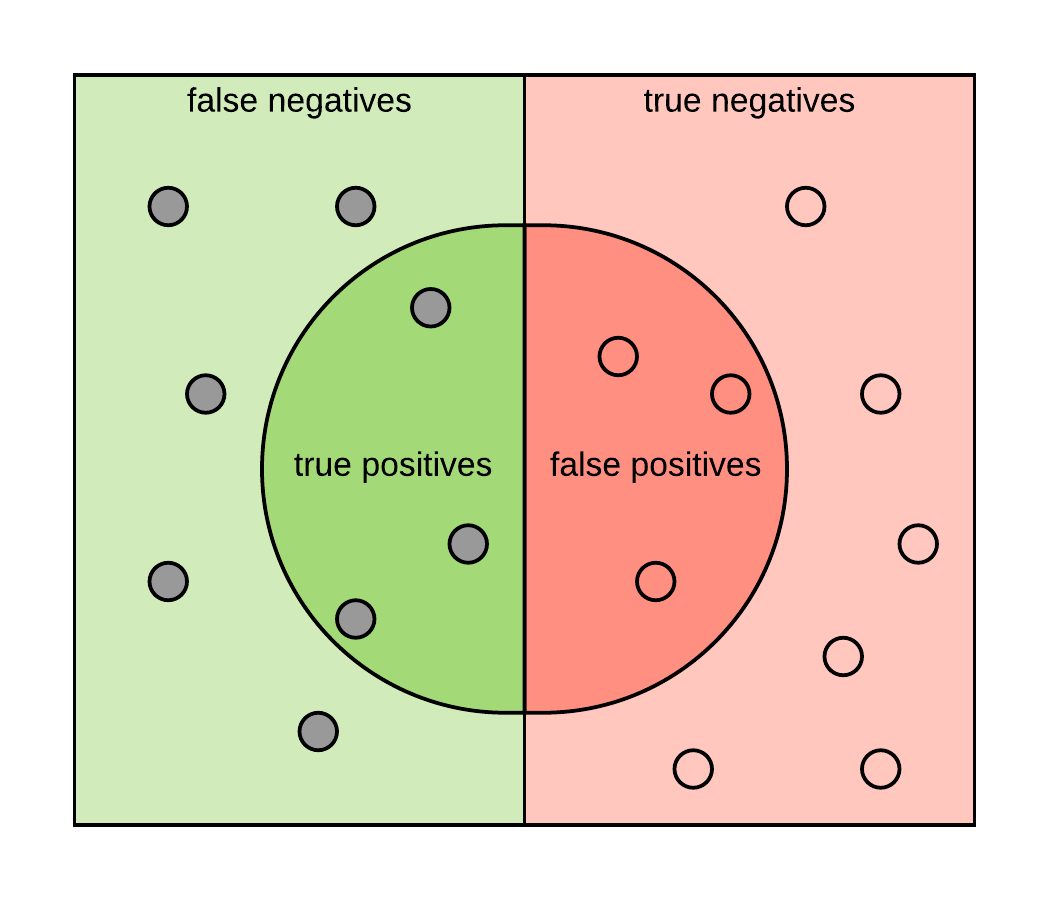
\includegraphics[width=0.8\textwidth]{PrecisionAndRecall}
	\caption{Precision and Recall visualisation. On the left side are the relevant elements.}
	\label{fig:PrecisionAndRecall}
\end{figure}

The reason to use precision and recall is, that both together create an accurate tool to measure the accuracy of an object detection algorithm. For further explanation of the used metrics, we use the abbreviation of the following terms:

\begin{enumerate}[label=]
    \item \textit{TP}: true positives
    \item \textit{FP}: false positives
    \item \textit{TN}: true negatives
    \item \textit{FN}: false negatives
\end{enumerate}

\paragraph{Precision}
\label{sub:Precision}

The precision score takes \textit{TP} and all retrieved documents (\textit{TP} and \textit{FP}), to calculate a score, which reflects the normalised amount of how many selected elements are relevant (Equation~\ref{eq:Precision}).

\begin{equation} \label{eq:Precision}
\begin{gathered}
precision = \frac{TP}{TP \cup  FP}
\end{gathered}
\end{equation}

\paragraph{Recall}
\label{sub:recall}

The recall score takes \textit{TP} and all positive documents (\textit{TP} and \textit{TN}), to calculate a score, which reflects the normalised amount of how many relevant elements are selected (Equation~\ref{eq:Recall}).

\begin{equation} \label{eq:Recall}
\begin{gathered}
recall = \frac{TP}{TP \cup  TN}
\end{gathered}
\end{equation}

\paragraph{F1 Score}
\label{sub:F1Score}
The \textit{F1} score combines the precision and recall with the harmonic mean (Equation~\ref{eq:F1Score}).

\begin{equation} \label{eq:F1Score}
\begin{gathered}
F_{1} = 2 * \frac{precision * recall}{precision + recall}
\end{gathered}
\end{equation}

